\documentclass[aspectratio=43,11pt]{beamer}

\usetheme{default}
\usecolortheme{default}
\setbeamertemplate{navigation symbols}{}
\setbeamertemplate{footline}{\hfill\footnotesize\color{gray}\insertframenumber\hspace{1em}\vspace{0.6em}}
\definecolor{accent}{HTML}{2b4bb0}
\definecolor{warm}{HTML}{dd3c20}
\definecolor{aggiemaroon}{RGB}{80,0,0}
\setbeamercolor{structure}{fg=aggiemaroon}
\setbeamercolor{frametitle}{fg=aggiemaroon}
\setbeamertemplate{itemize items}{\textbullet}
\usepackage{booktabs,amsmath,graphicx,xcolor,listings}
\lstset{basicstyle=\ttfamily\footnotesize,keywordstyle=\color{accent},commentstyle=\color{gray},
        columns=fullflexible,keepspaces=true,showstringspaces=false}
\newcommand{\hl}[1]{\textcolor{warm}{\textbf{#1}}}
\newcommand{\logit}{\log\!\left(\frac{\pi}{1-\pi}\right)}

\title{Decision and Risk Analysis}
\subtitle{Lecture 12: \textbf{Logistic Regression}}
\author{}
%\institute{Industrial \& Systems Engineering, Texas A\&M University}
\date{\color{aggiemaroon}{DAEN 427 / ISEN 427 / ISEN 627 - Fall 2026\\
      \textbf{Alexander Abuabara}}}
\titlegraphic{\vfill 
\includegraphics[height=1.2cm]{TAMU_logo.png}}

\begin{document}

\begin{frame}[plain]
  \titlepage
\end{frame}

% ---------------- HOOK ----------------
\begin{frame}{Let's start with a bet \dots}
  \centering
  \Large It's 9 AM\ in Perth, Australia.\\[0.3em]
  Humidity is \hl{99\%}.\\[1em]
  \normalsize
  \textbf{Will it rain tomorrow?}\\[0.8em]
  \begin{tabular}{l}
    (A) Almost surely, $>90\%$\\[0.2em]
    (B) A coin flip, $\approx 50\%$\\[0.2em]
    (C) Unlikely, $<20\%$
  \end{tabular}\\[1.2em]
  \small Hold on to your answer --- the data will settle it by the end of class.\\[0.6em]
  \footnotesize\color{gray} Should you carry an umbrella? (Well, that's a \emph{different} question)
\end{frame}

\begin{frame}{}
  \begin{enumerate}
    \setlength\itemsep{0.6em}
    \item Why a binary $Y$ needs a new model
    \item Probability $\leftrightarrow$ odds $\leftrightarrow$ log-odds
    \item The Bayesian logistic regression model + priors
    \item Posterior: what humidity tells us about rain
    \item From probabilities to \emph{decisions}: classification \& cutoffs
    \item Adding predictors, comparing models
  \end{enumerate}
\end{frame}

% ---------------- SETTING ----------------
\begin{frame}{The running example: rain in Perth}
  \begin{columns}[T]
    \column{0.55\textwidth}
    \textbf{Response}\\
    $Y = 1$ if it rains tomorrow,\\$0$ otherwise\\[0.8em]
    \textbf{Predictors}
    \begin{itemize}
      \item $X_1$: today's 9 am\ humidity (\%)
      \item $X_2$: today's 3 pm\ humidity (\%)
      \item $X_3$: did it rain today?
    \end{itemize}
    \textbf{Data}: \texttt{weather\_perth}, 1{,}000 days
    \column{0.42\textwidth}
    \begin{block}{Prior knowledge}
      On a typical day in Perth, the chance of rain is about \hl{20\%}.
    \end{block}
    \vspace{0.5em}
    \small Same Bayesian recipe as always:\\
    \emph{prior} $+$ \emph{data} $\Rightarrow$ \emph{posterior}.\\
    Only the data model changes.
  \end{columns}
\end{frame}

\begin{frame}{Why not just use Normal regression?}
  \centering
  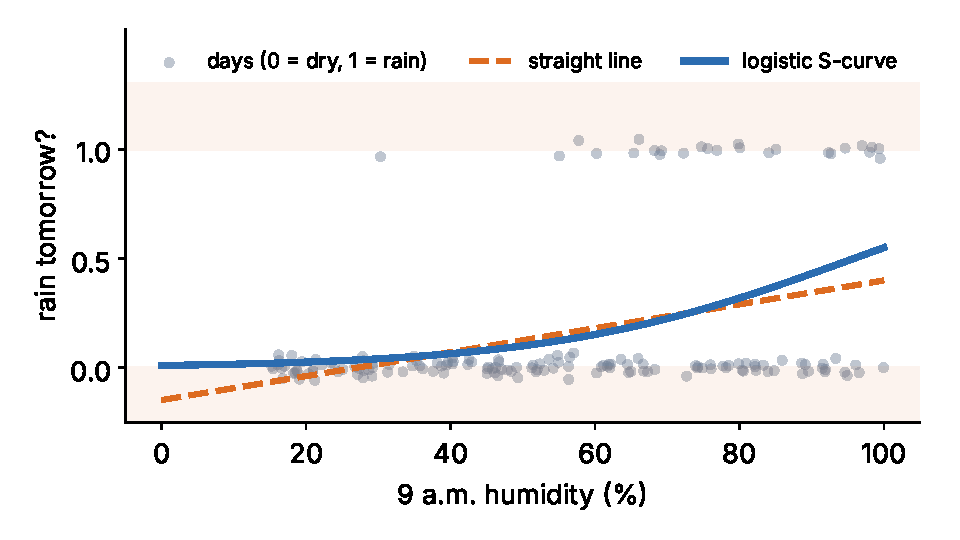
\includegraphics[width=0.92\textwidth]{line_vs_s.pdf}\\[-0.2em]
  \small A straight line predicts ``probabilities'' below 0 and above 1 (shaded).\\
  We need a curve that \hl{stays between 0 and 1}.
\end{frame}

% ---------------- ODDS ----------------
\begin{frame}{Odds: a familiar idea from sports and betting}
  \[
    \text{odds} = \frac{\pi}{1-\pi}, \qquad \pi = \frac{\text{odds}}{1+\text{odds}}
  \]
  \vspace{-0.4em}
  \begin{center}
  \begin{tabular}{ccl}
    \toprule
    $\pi$ & odds & meaning\\ \midrule
    $2/3$ & $2$ & rain twice as likely as no rain\\
    $1/2$ & $1$ & even chance\\
    $1/3$ & $1/2$ & rain half as likely as no rain\\
    $0.8$ & $4$ & ``4 to 1'' in favor\\ \bottomrule
  \end{tabular}
  \end{center}
  \vspace{0.3em}
  \centering
  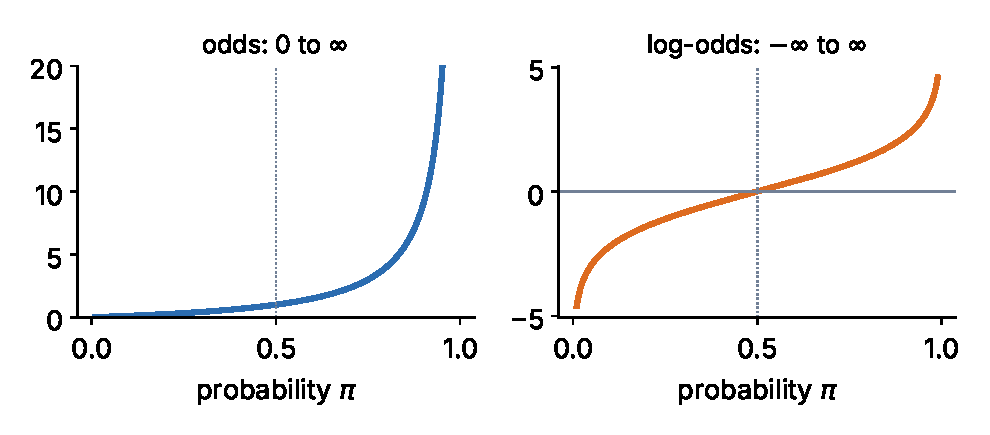
\includegraphics[width=0.72\textwidth]{scales.pdf}
\end{frame}

\begin{frame}{Three ways to say the same thing}
  \begin{center}
  \begin{tabular}{lcc}
    \toprule
    scale & range & 50/50 point\\ \midrule
    probability $\pi$ & $[0,1]$ & $0.5$\\
    odds $\pi/(1-\pi)$ & $[0,\infty)$ & $1$\\
    log-odds $\log\big(\pi/(1-\pi)\big)$ & $(-\infty,\infty)$ & $0$\\ \bottomrule
  \end{tabular}
  \end{center}
  \vspace{0.8em}
  \begin{block}{}
    Log-odds can be \emph{any} real number: so it's safe to model it with a line
    $\beta_0 + \beta_1 X$, just like in Normal regression.
  \end{block}
  \vspace{0.4em}
  \small\textbf{Quick check:} our prior of 20\% rain $\Rightarrow$ odds $= 0.2/0.8 = 0.25$
  $\Rightarrow$ log-odds $= \log(0.25) \approx \hl{-1.4}$. Remember this number!
\end{frame}

% ---------------- MODEL ----------------
\begin{frame}{The logistic regression model}
  \textbf{Data model} (Bernoulli: $Y$ is 0 or 1)
  \[ Y_i \mid \beta_0,\beta_1 \;\overset{ind}{\sim}\; \text{Bern}(\pi_i) \]
  \textbf{Link function} (logit: connects $\pi_i$ to a line)
  \[ \log\!\left(\frac{\pi_i}{1-\pi_i}\right) = \beta_0 + \beta_1 X_{i1} \]
  \textbf{Back to probability}
  \[ \pi_i = \frac{e^{\beta_0+\beta_1 X_{i1}}}{1+e^{\beta_0+\beta_1 X_{i1}}} \]
  \vspace{-0.3em}
  \begin{center}\small
  \fbox{\parbox{0.85\textwidth}{\centering
  line on the \hl{log-odds} scale \;$\Longleftrightarrow$\; S-curve on the \hl{probability} scale}}
  \end{center}
\end{frame}

\begin{frame}{Reading the coefficients}
  \begin{itemize}
    \setlength\itemsep{0.5em}
    \item $\beta_0$: log-odds when $X = 0$; \quad $e^{\beta_0}$: odds when $X=0$
    \item $\beta_1$: change in \emph{log-odds} per 1-unit increase in $X$
    \item $e^{\beta_1}$: \hl{multiplicative} change in \emph{odds} per 1-unit increase in $X$
  \end{itemize}
  \vspace{0.5em}
  \begin{exampleblock}{Example: $\log(\text{odds}) = -4 + 0.1\,X$}
    \begin{itemize}
      \item At 0\% humidity: odds $= e^{-4} = 0.018$, so $\pi \approx 0.018$
      \item $e^{0.1} = 1.11$: each extra humidity point \\
            multiplies the odds of rain by 1.11 (\hl{+11\%})
    \end{itemize}
  \end{exampleblock}
  \vspace{0.3em}
  \small\color{gray} Careful: ``+11\% odds'' is \emph{not} ``+11 percentage points of probability.''
\end{frame}

% ---------------- PRIORS ----------------
\begin{frame}{Tuning the priors}
  \textbf{Intercept} (centered at typical humidity)
  \[ \beta_{0c} \sim N(-1.4,\; 0.7^2) \]
  \vspace{-0.6em}
  \begin{itemize}
    \item Center $-1.4 = \log(0.2/0.8)$: our 20\% rain belief
    \item $\pm 2$ sd $\Rightarrow$ log-odds $\in(-2.8, 0)$ $\Rightarrow$ $\pi \in (0.06, 0.50)$
  \end{itemize}
  \vspace{0.3em}
  \textbf{Slope}
  \[ \beta_1 \sim N(0.07,\; 0.035^2) \]
  \vspace{-0.6em}
  \begin{itemize}
    \item We expect humidity to \emph{increase} rain chances
    \item $\pm 2$ sd $\Rightarrow$ $\beta_1 \in (0, 0.14)$ $\Rightarrow$ odds go up \hl{0\% to 15\%} per point
  \end{itemize}
\end{frame}

\begin{frame}{Do our priors make sense? Simulate them!}
  \centering
  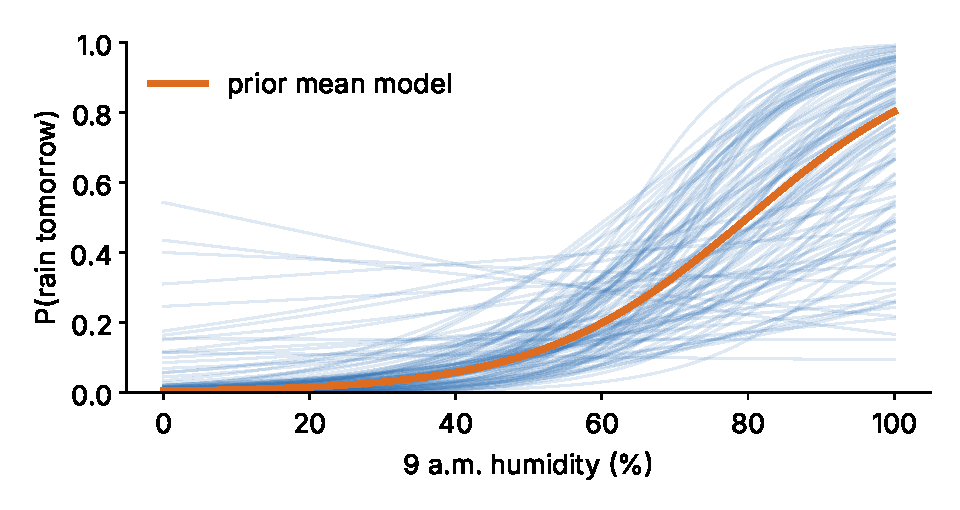
\includegraphics[width=0.92\textwidth]{prior_curves.pdf}\\
  \small 100 plausible models drawn from the prior.\\
  All agree: more humidity, more rain.
  But they disagree on \emph{how much}. Simulated rain rates range from about 5\% to 50\%.
\end{frame}

% ---------------- POSTERIOR ----------------
\begin{frame}{What the data say: the posterior}
  \begin{center}
  \begin{tabular}{lcc}
    \toprule
    80\% posterior interval & log-odds scale & odds scale \\ \midrule
    intercept $\beta_0$ & $(-5.09,\,-4.13)$ & $(0.006,\,0.016)$\\
    humidity $\beta_1$ & $(0.041,\,0.055)$ & $(1.042,\,1.056)$\\ \bottomrule
  \end{tabular}
  \end{center}
  \vspace{0.6em}
  \begin{itemize}
    \setlength\itemsep{0.5em}
    \item Each humidity point raises the odds of rain by \hl{4.2\% to 5.6\%}
    \item 15 more humidity points $\Rightarrow$ odds roughly \hl{double}\\($\times1.86$ to $\times2.28$)
    \item The slope is \emph{smaller} than our prior guess (0.07): the data humbled us
  \end{itemize}
\end{frame}

\begin{frame}{Posterior plausible models}
  \centering
  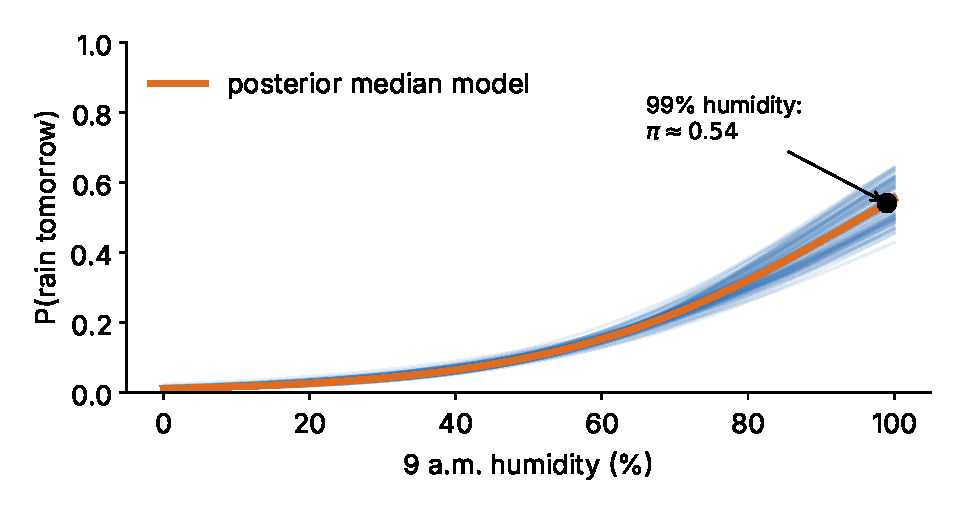
\includegraphics[width=0.92\textwidth]{posterior_curves.pdf}\\
  \small Much less uncertainty than the prior.\\
  Even at the highest humidity,
  rain is only a bit more likely than not.\\
  {\footnotesize\color{gray}(curves drawn from an approximation to the book's posterior)}
\end{frame}

\begin{frame}{Back to our bet: 99\% humidity}
  \textbf{One posterior draw:} $\beta_0 = -4.244,\ \beta_1 = 0.0446$
  \[
    \log(\text{odds}) = -4.244 + 0.0446(99) = 0.166
    \Rightarrow \pi = \frac{e^{0.166}}{1+e^{0.166}} \approx 0.54
  \]
  \textbf{All 20{,}000 draws:} simulate $Y \sim \text{Bern}(\pi)$ for each one
  \begin{center}
    \begin{tabular}{cc}
      \toprule
      rain ($Y=1$) & no rain ($Y=0$)\\ \midrule
      10{,}804 \;(54\%) & 9{,}196 \;(46\%)\\ \bottomrule
    \end{tabular}
  \end{center}
  \vspace{0.3em}
  \begin{alertblock}{Answer to the initial question!!}
    \textbf{(B)} --- about a coin flip!\\
    High humidity helps, but it's far from a guarantee.
  \end{alertblock}
\end{frame}

% ---------------- CLASSIFICATION ----------------
\begin{frame}{From probability to decision: classification}
  \begin{block}{Classification rule with cutoff $c$}
    Let $p$ = proportion of posterior predictions with $Y = 1$.\\[0.2em]
    \centering If $p \ge c$, classify $\hat Y = 1$ (rain); \; otherwise $\hat Y = 0$.
  \end{block}
  \vspace{0.6em}
  \begin{itemize}
    \setlength\itemsep{0.5em}
    \item Default: $c = 0.5$. At 99\% humidity, $p = 0.54 \Rightarrow$ predict \hl{rain}
    \item But the cutoff is a \emph{value judgment}, not a statistical fact:
    \begin{itemize}
      \item Hate getting wet? Use a \hl{low} cutoff, e.g.\ $c = 0.25$
      \item Hate carrying an umbrella? Use a \hl{high} cutoff, e.g.\ $c = 0.75$
    \end{itemize}
  \end{itemize}
\end{frame}

\begin{frame}{How good are our predictions? ($c = 0.5$)}
  \begin{columns}[c]
    \column{0.52\textwidth}
    \centering\small
    \begin{tabular}{@{}l|cc|c@{}}
      & $\hat Y=0$ & $\hat Y=1$ & total\\ \hline
      no rain & 803 & 11 & 814\\
      rain & \hl{172} & 14 & 186\\
    \end{tabular}\\[0.4em]
    \footnotesize in-sample, 1{,}000 days
    \column{0.46\textwidth}
    \small
    \textbf{Accuracy}: $\frac{803+14}{1000} = 81.7\%$\\[0.5em]
    \textbf{Specificity} (true neg.\ rate):\\ $\frac{803}{814} = 98.7\%$\\[0.5em]
    \textbf{Sensitivity} (true pos.\ rate):\\ $\frac{14}{186} = \hl{7.5\%}$
  \end{columns}
  \vspace{1em}
  \begin{alertblock}{Looks great \dots~until you look closer}
    We miss 172 of 186 rainy days! A lazy rule ``\emph{never} predict rain'' would score 81.4\%.
    Accuracy alone can be misleading when one outcome is rare.
  \end{alertblock}
\end{frame}

\begin{frame}{Moving the cutoff: a trade-off}
  \centering
  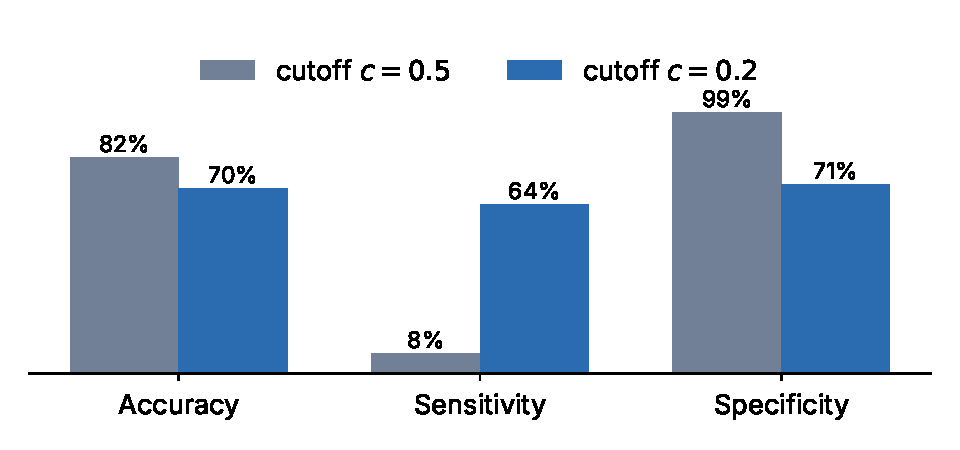
\includegraphics[width=0.9\textwidth]{cutoff.pdf}\\[0.3em]
  \raggedright\small
  \begin{itemize}
    \item Lower cutoff $\Rightarrow$ catch more rainy days (sensitivity $\uparrow$), more false alarms (specificity $\downarrow$)
    \item 10-fold cross-validation at $c=0.2$: sens.\ 0.65, spec.\ 0.72, acc.\ 0.71 --- close to in-sample, so little overfitting
  \end{itemize}
\end{frame}

% ---------------- MODEL 2 ----------------
\begin{frame}{Adding more predictors}
  \[ \log(\text{odds}) = \beta_0 + \beta_1\,\text{hum9am} + \beta_2\,\text{hum3pm} + \beta_3\,\text{rainToday} \]
  \begin{center}\small
  \begin{tabular}{lrc}
    \toprule
    term & median & 80\% interval\\ \midrule
    intercept & $-5.46$ & $(-6.08,\,-4.85)$\\
    humidity 9 a.m. & $-0.007$ & $(-0.016,\,0.003)$\\
    humidity 3 p.m. & $0.080$ & $(0.069,\,0.091)$\\
    rain today & $1.15$ & $(0.87,\,1.44)$\\ \bottomrule
  \end{tabular}
  \end{center}
  \begin{itemize}
    \item Rain today: odds $\times\, e^{1.15} \approx \hl{3.2}$ --- more than triple!
    \item Morning humidity \emph{loses} its effect: its information overlaps
          with afternoon humidity and rain today
  \end{itemize}
\end{frame}

\begin{frame}{Which model wins?}
  \begin{center}
  \begin{tabular}{lccc}
    \toprule
    10-fold CV, $c=0.2$ & sensitivity & specificity & accuracy\\ \midrule
    Model 1 (hum9am) & 0.65 & 0.72 & 0.71\\
    Model 2 (three predictors) & \hl{0.75} & \hl{0.81} & \hl{0.80}\\ \bottomrule
  \end{tabular}
  \end{center}
  \vspace{0.6em}
  \begin{itemize}
    \setlength\itemsep{0.4em}
    \item Model 2 is better on \emph{every} metric
    \item ELPD difference: $-80.2$ (SE 13.5) --- about 6 SEs in favor of Model 2
  \end{itemize}
  \vspace{0.5em}
  \small\color{gray} Lesson: a single noisy predictor rarely tells the whole story.
\end{frame}

\begin{frame}[fragile]{In R: just a few lines}
\begin{lstlisting}[language=R]
library(bayesrules); library(rstanarm)
data(weather_perth)

rain_model_1 <- stan_glm(
  raintomorrow ~ humidity9am, data = weather_perth,
  family = binomial, # logistic!
  prior_intercept = normal(-1.4, 0.7),
  prior           = normal(0.07, 0.035),
  chains = 4, iter = 5000*2, seed = 84735)

posterior_interval(rain_model_1, prob = 0.80)
exp(posterior_interval(rain_model_1, prob = 0.80)) # odds scale

classification_summary(model = rain_model_1,
  data = weather_perth, cutoff = 0.2)
classification_summary_cv(model = rain_model_1,
  data = weather_perth, cutoff = 0.2, k = 10)
\end{lstlisting}
  \footnotesize\color{gray} Add \texttt{prior\_PD = TRUE} to simulate from the prior only!
\end{frame}

\begin{frame}{Take-home messages}
  \begin{enumerate}
    \setlength\itemsep{0.6em}
    \item Binary $Y$ $\Rightarrow$ \hl{Bernoulli} data model + \hl{logit} link
    \item Model a line on the log-odds scale; read results as odds ($e^{\beta}$) or probabilities
    \item Priors are tuned on familiar scales (20\% rain $\to -1.4$), then checked by simulation
    \item Classification needs a \hl{cutoff} --- choose it based on what errors cost you
    \item Judge models by sensitivity, specificity, and accuracy --- ideally cross-validated
  \end{enumerate}
\end{frame}

% ---------------- PRACTICE ----------------
\begin{frame}{Practice question 1: passing the exam}
  A posterior median model for passing an exam ($Y=1$) based on hours studied $X$:
  \[ \log(\text{odds of passing}) = -3 + 0.25\,X \]
  \begin{enumerate}[(a)]
    \setlength\itemsep{0.6em}
    \item Interpret $e^{0.25}$ in plain words.
    \item What is the probability of passing after 12 hours of study?
    \item \dots and after 16 hours?
  \end{enumerate}
  \vspace{1em}
  \centering\small\color{gray} Take 1-2 minutes with your neighbor.
\end{frame}

\begin{frame}{Answers}
  \begin{enumerate}[(a)]
    \setlength\itemsep{0.8em}
    \item $e^{0.25} \approx 1.28$: each extra hour of study multiplies the
          \emph{odds} of passing by 1.28 --- a \hl{28\% increase in odds}.
    \item $X = 12$: \; $\log(\text{odds}) = -3 + 0.25(12) = 0$\\[0.2em]
          odds $= e^0 = 1$ \;$\Rightarrow$\; $\pi = \frac{1}{1+1} = \hl{0.50}$
    \item $X = 16$: \; $\log(\text{odds}) = -3 + 0.25(16) = 1$\\[0.2em]
          odds $= e^1 \approx 2.72$ \;$\Rightarrow$\; $\pi = \frac{2.72}{3.72} \approx \hl{0.73}$
  \end{enumerate}
  \vspace{0.6em}
  \small\color{gray} Note: 4 more hours added 23 percentage points here, but the same 4 hours
  would add less near $\pi = 0$ or $\pi = 1$. The S-curve is not a straight line!
\end{frame}

\begin{frame}{Practice question 2: a spam filter}
  A Bayesian logistic spam filter, cutoff $c = 0.5$, tested on 1{,}000 emails:
  \begin{center}
  \begin{tabular}{l|cc|c}
    & predicted not spam & predicted spam & total\\ \hline
    not spam & 855 & 45 & 900\\
    spam & 20 & 80 & 100\\
  \end{tabular}
  \end{center}
  \begin{enumerate}[(a)]
    \setlength\itemsep{0.5em}
    \item Compute accuracy, sensitivity, and specificity.
    \item Missing an important email is costly.\\
    Should we \emph{raise} or \emph{lower} the cutoff? What gets worse?
  \end{enumerate}
\end{frame}

\begin{frame}{Answers}
  \begin{enumerate}[(a)]
    \setlength\itemsep{0.6em}
    \item \textbf{Accuracy} $= \frac{855+80}{1000} = \hl{93.5\%}$\\[0.2em]
          \textbf{Sensitivity} $= \frac{80}{100} = \hl{80\%}$ \;(spam caught)\\[0.2em]
          \textbf{Specificity} $= \frac{855}{900} = \hl{95\%}$ \;(real email let through)
    \item \textbf{Raise} the cutoff (e.g.\ $c = 0.8$): only flag emails we're very sure are spam.
          \begin{itemize}
            \item Specificity $\uparrow$ --- fewer real emails sent to the spam folder
            \item Sensitivity $\downarrow$ --- more spam slips into your inbox
          \end{itemize}
  \end{enumerate}
  \vspace{0.5em}
  \begin{block}{}
    The model gives probabilities;\\
    \emph{you} decide the cutoff based on which mistake hurts more :)
  \end{block}
\end{frame}

\end{document}